\section{Simulation Analysis}
\label{sec:simulation}

In this section we wrote a \textit{Ngspice} script to simulate the audio
amplifier circuit, using the transistor models provided in the .net script
(NPN for the gain stage and PNP for the output stage).
Finally we measured the output voltage gain in the passband,
the lower and upper 3dB cut off frequencies and the input and output
impedances.


The circuit studied had a cost of 9600.608 MU. Much of the cost can be
attributable to the capacitors used.


\begin{figure*}[h]
    \centering
    \begin{subfigure}{0.23\textwidth}
        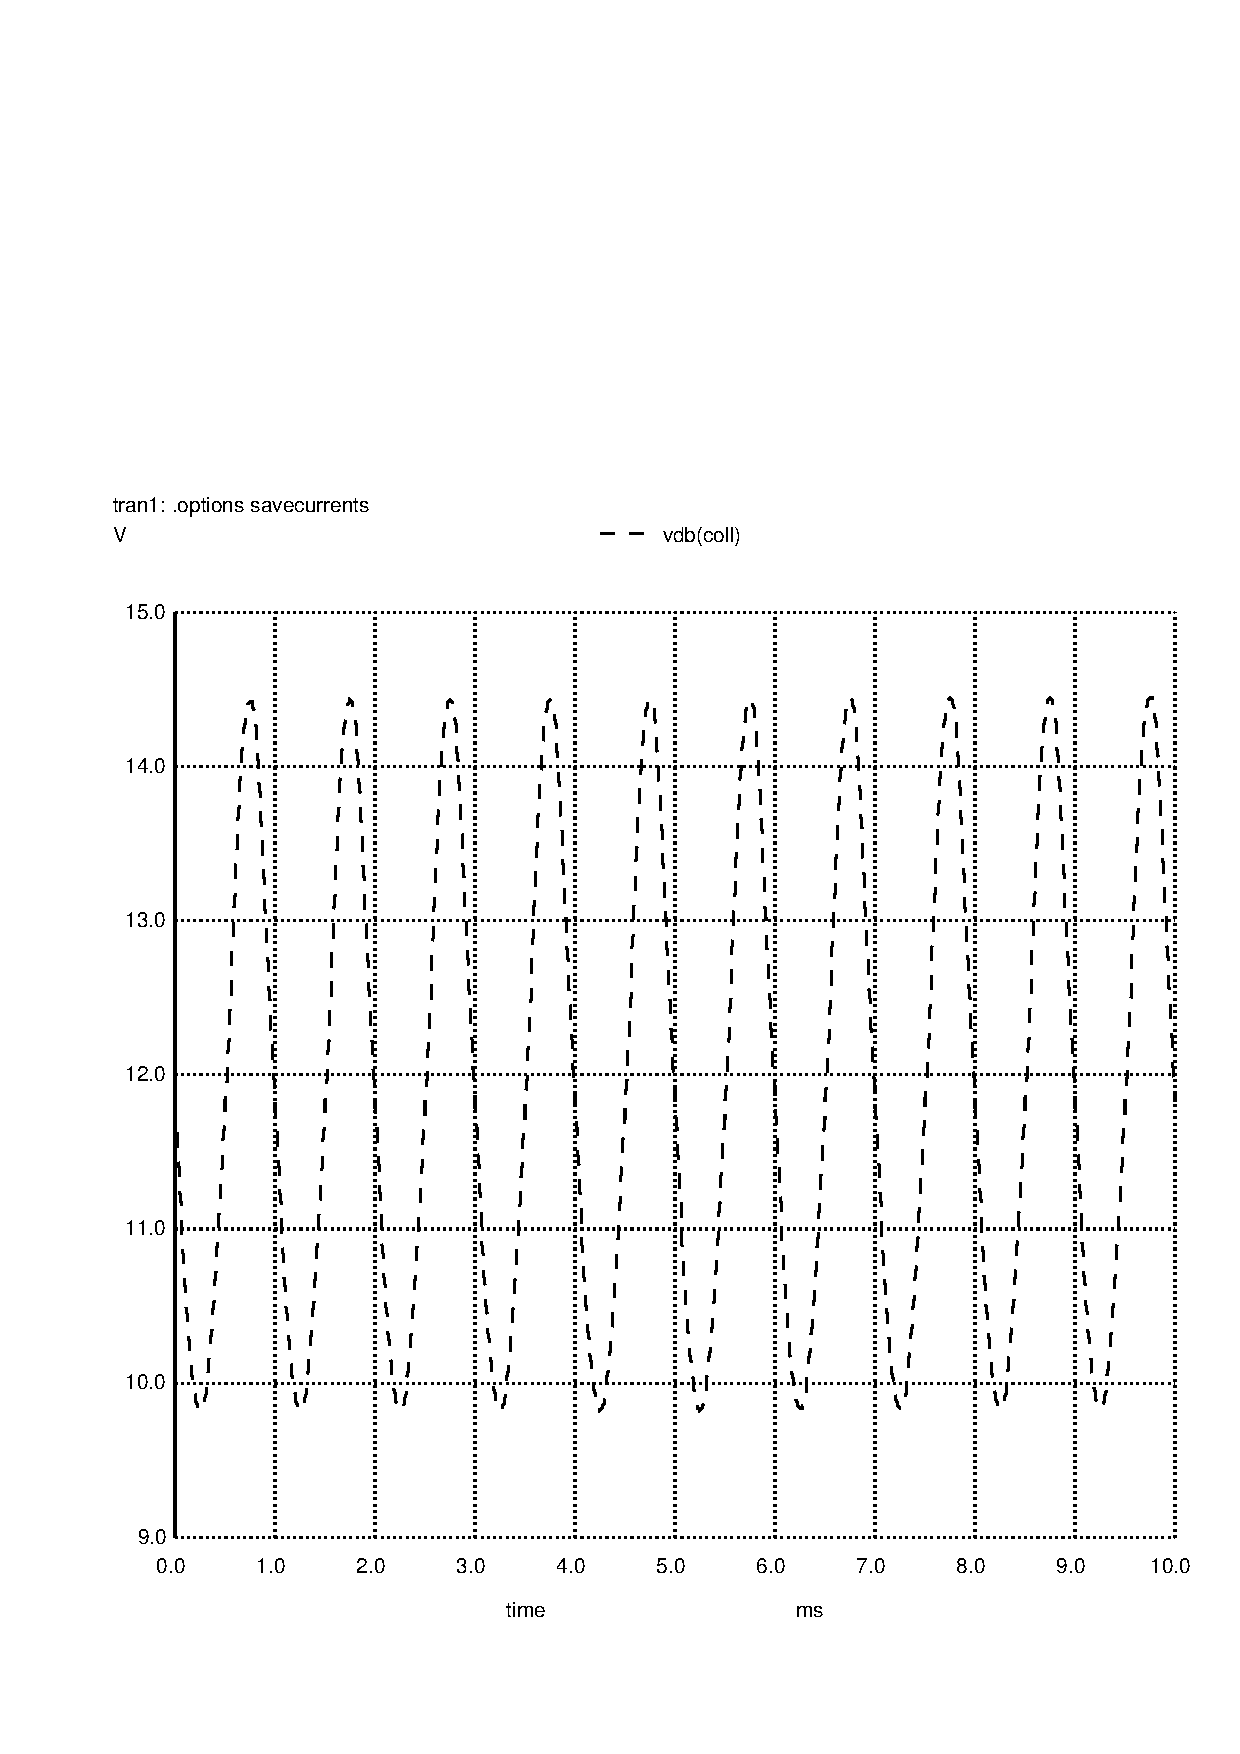
\includegraphics[width=\linewidth, clip]{vo1.pdf}
        \label{fig:output1}
    \end{subfigure}
    \begin{subfigure}{0.23\textwidth}
        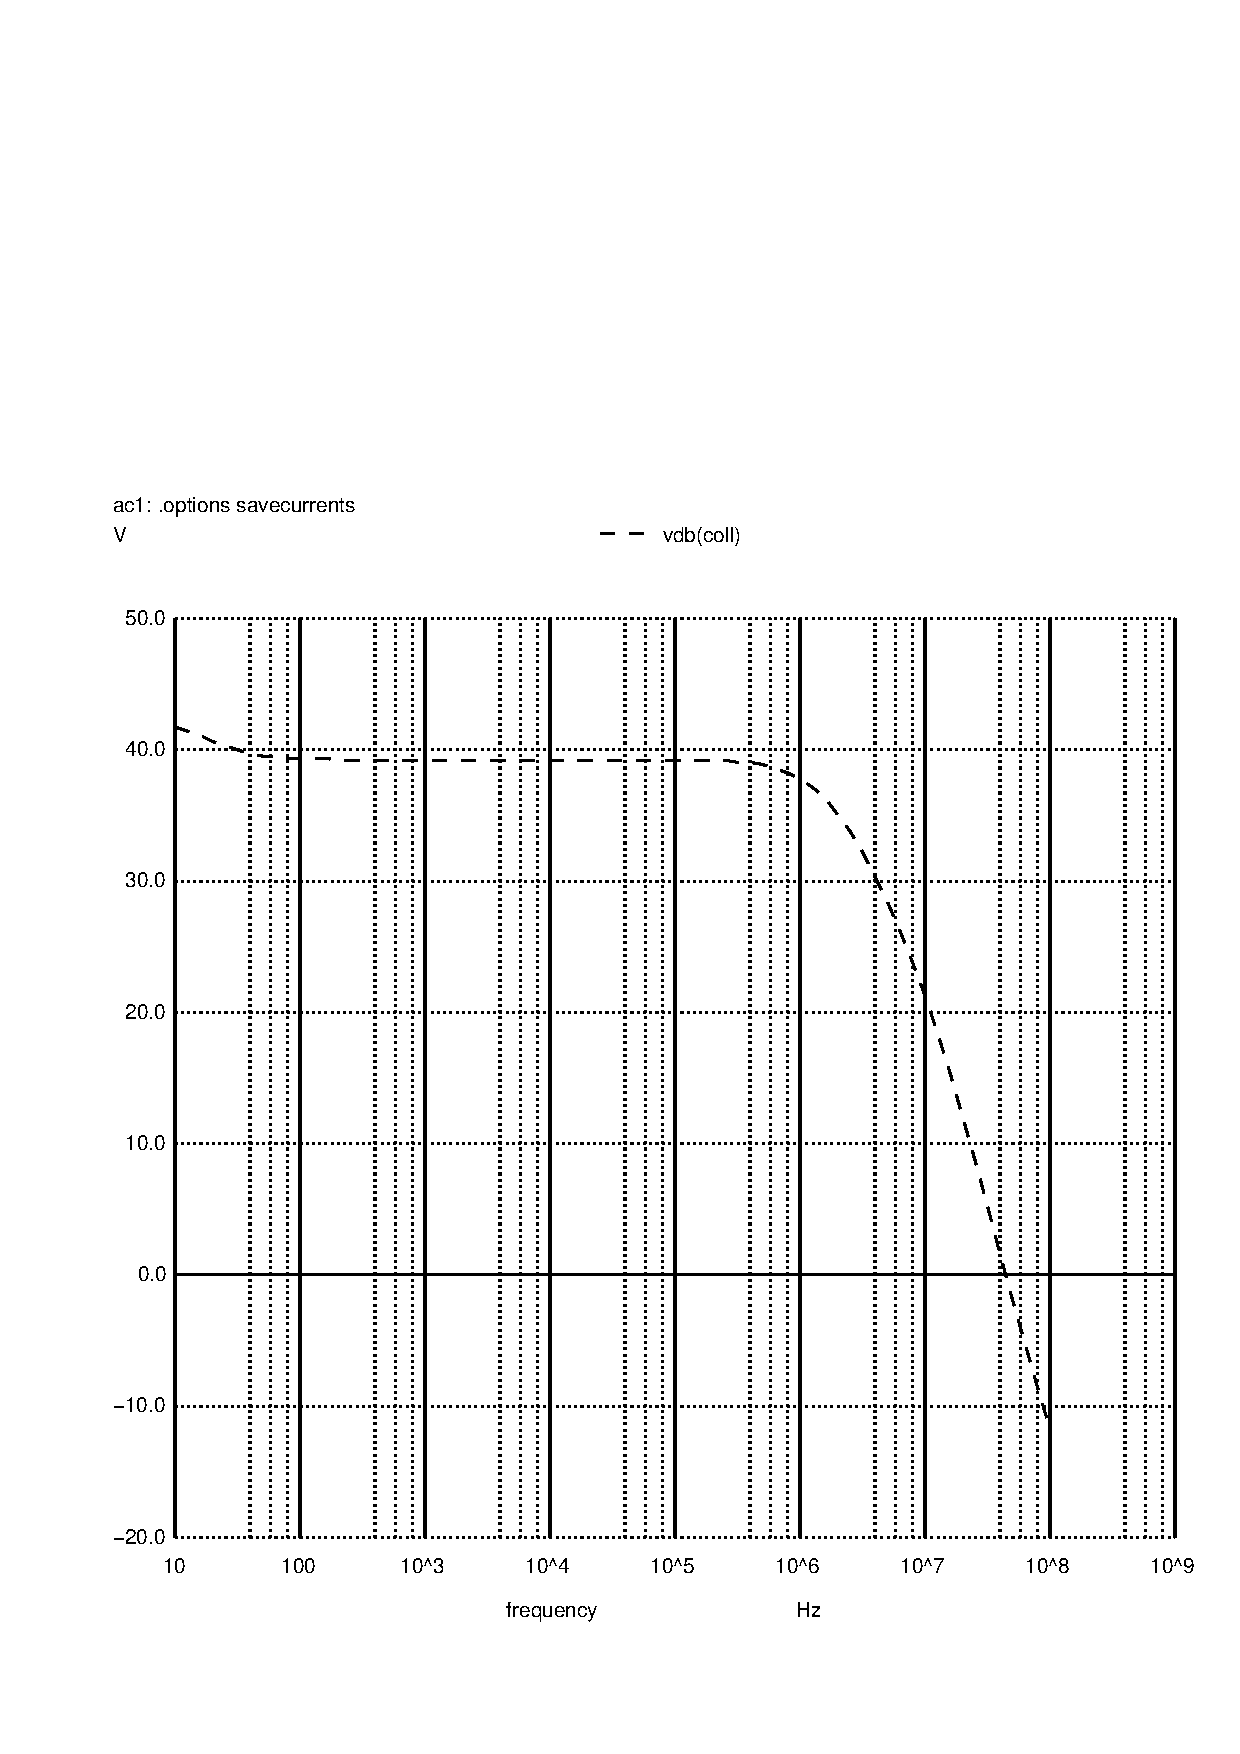
\includegraphics[width=\linewidth, clip]{vo1f.pdf}
        \label{fig:output2}
    \end{subfigure}
    \caption{\small $V_Out - 12$ - measure of the output DC deviation + AC component (left - simulation; right - theoretical )}
    \label{output_deviation}
\end{figure*}

\begin{figure*}[h]
    \centering
    \begin{subfigure}{0.23\textwidth}
        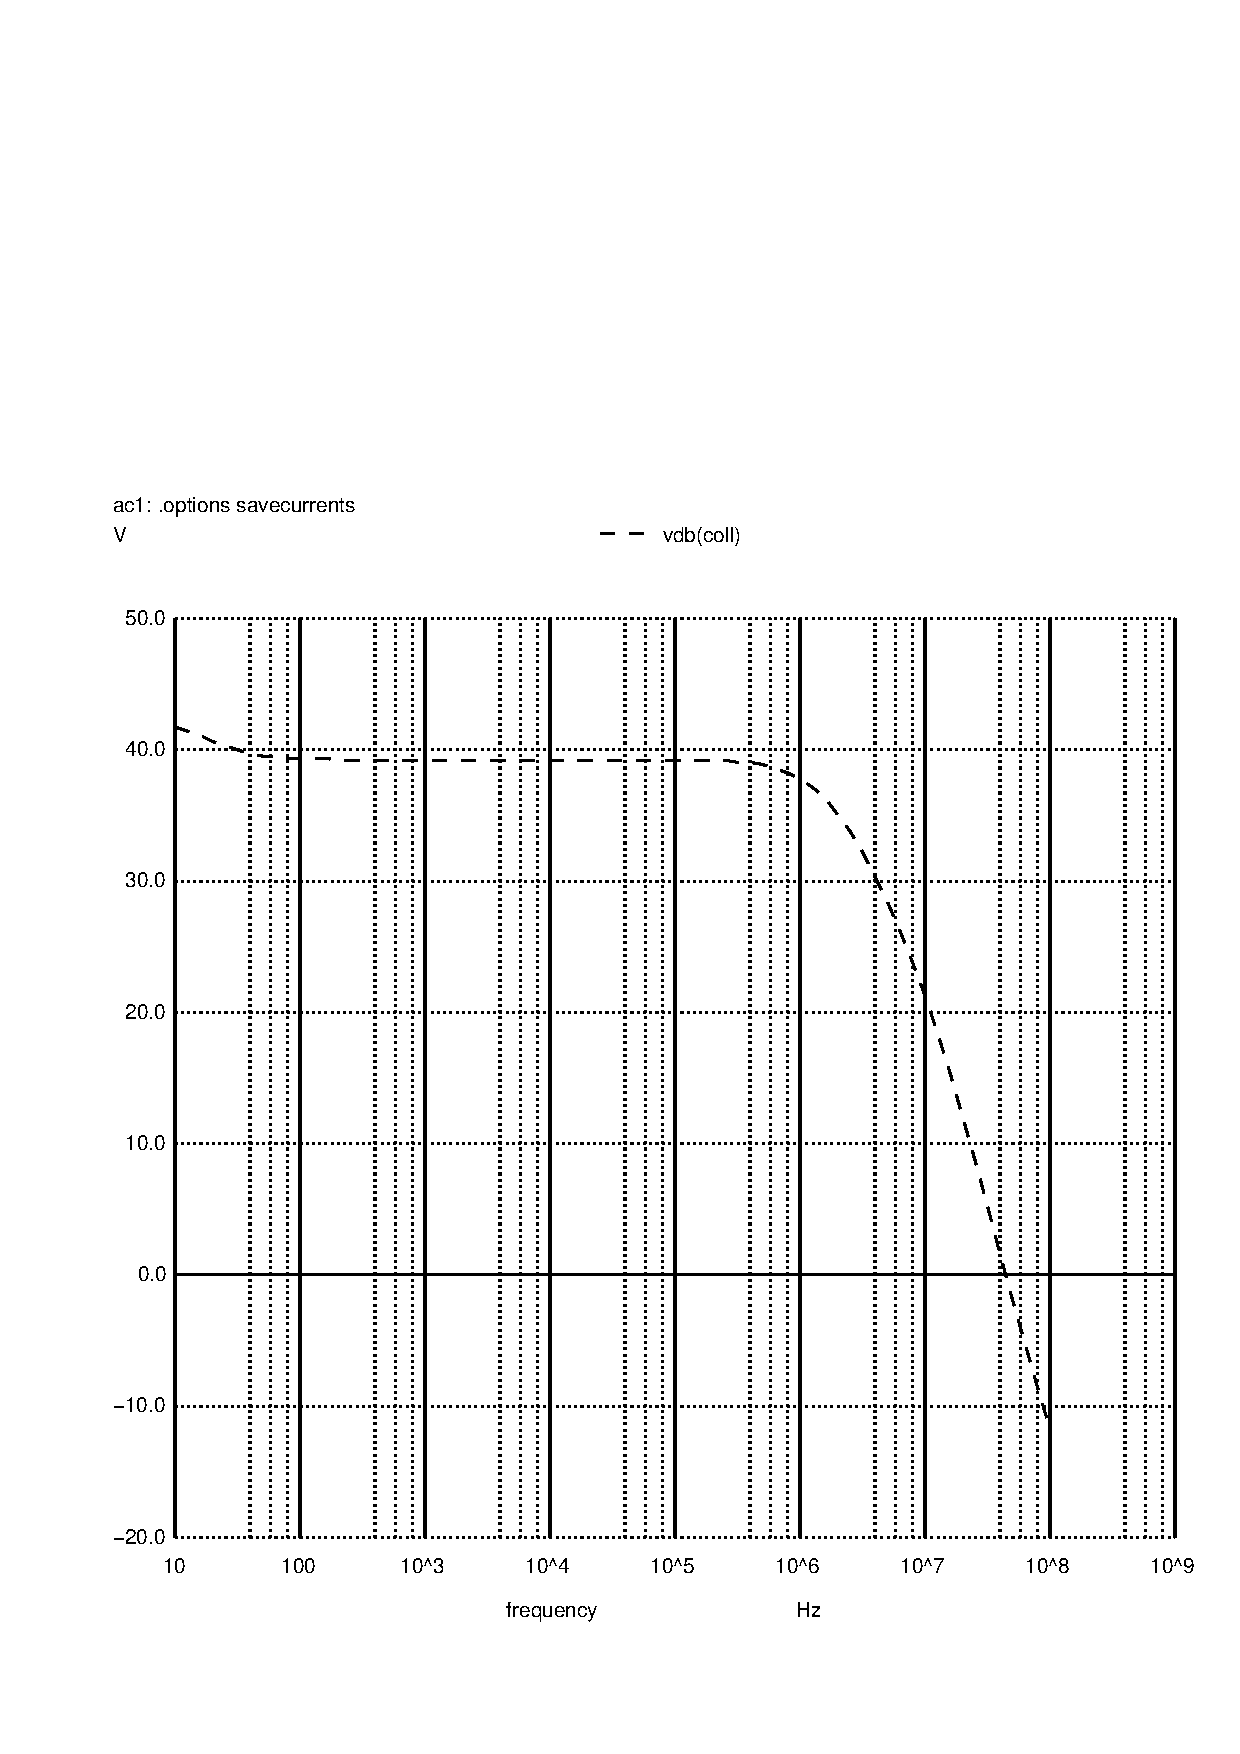
\includegraphics[width=\linewidth, clip]{vo2f.pdf}
        \label{fig:output1}
    \end{subfigure}
    \begin{subfigure}{0.23\textwidth}
        \includegraphics[width=\linewidth, clip]{gainACtotal.eps}
        \label{fig:output2}
    \end{subfigure}
    \caption{\small $V_Out - 12$ - measure of the output DC deviation + AC component (left - simulation; right - theoretical )}
    \label{output_deviation}
\end{figure*}

% \begin{figure}
%     \centering
%     \begin{subfigure}{.5\textwidth}
%         \centering
%         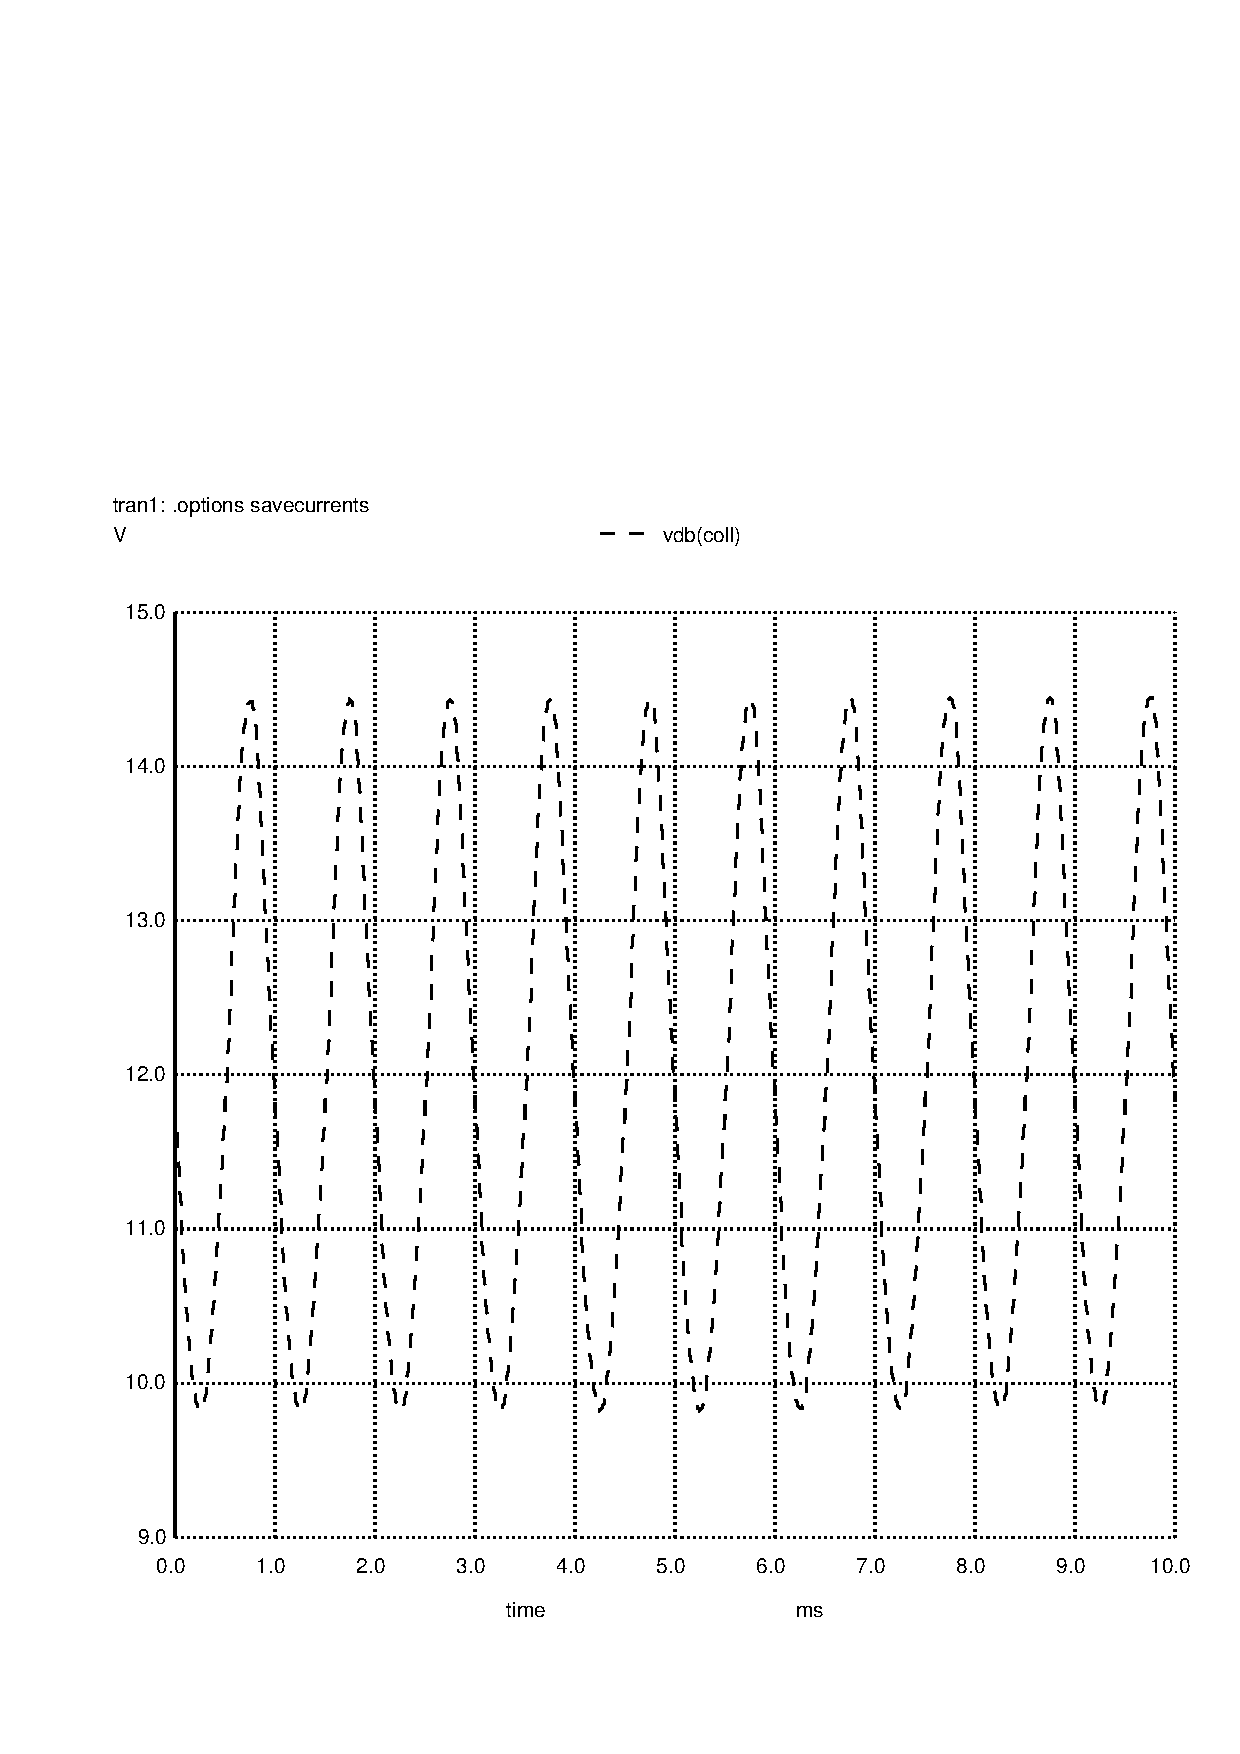
\includegraphics[width=.4\linewidth]{vo1.pdf}
%         \caption{A subfigure}
%         \label{fig:sub1}
%     \end{subfigure}%
%     \begin{subfigure}{.5\textwidth}
%         \centering
%         \includegraphics[width=.4\linewidth]{gainACtotal.eps}
%         \caption{A subfigure}
%         \label{fig:sub2}
%     \end{subfigure}
%     \caption{A figure with two subfigures}
%     \label{fig:test}
% \end{figure}


\begin{table}
    \parbox{.45\linewidth}{
        \centering
        \begin{tabular}{|c|c|}
            \hline
            {\bf Name} & {\bf Value [A or V]} \\ \hline
            VEQ & 2.400000e+00\\ \hline
IB1 & 5.004416e-05\\ \hline
IC1 & 8.942891e-03\\ \hline
VEQ & 8.992935e-03\\ \hline
VE1 & 8.992935e-01\\ \hline
V01 & 3.057109e+00\\ \hline
VCE & 2.157816e+00\\ \hline

        \end{tabular}
        \label{tab:GainStage_OP}
        \caption{Results of the DC analysis applied to the Gain Stage circuit}
    }
    \hfill
    \parbox{.45\linewidth}{
        \centering
        \begin{tabular}{|c|c|}
            {\bf Name} & {\bf Value [A or V]} \\ \hline
            @gib[i] & -2.65517e-04\\ \hline
@id[current] & 1.025904e-03\\ \hline
@r1[i] & -2.53670e-04\\ \hline
@r2[i] & -2.65517e-04\\ \hline
@r3[i] & -1.18476e-05\\ \hline
@r4[i] & 1.220737e-03\\ \hline
@r5[i] & -1.29142e-03\\ \hline
@r6[i] & 9.670671e-04\\ \hline
@r7[i] & 9.670671e-04\\ \hline
v(1) & -7.95657e+00\\ \hline
v(2) & 3.950179e+00\\ \hline
v(3) & -3.64391e-02\\ \hline
v(4) & -4.95541e+00\\ \hline
v(5) & -6.94792e+00\\ \hline
v(6) & -5.78231e-01\\ \hline
v(7) & 2.284139e-01\\ \hline
v(8) & -4.95541e+00\\ \hline

            \hline
        \end{tabular}
        \label{tab:Spice_OP}
        \caption{Results of the OP analysis applied to the whole circuit by using the Ngspice}
    }
    \hfill
    \parbox{.45\linewidth}{
        \centering
        \begin{tabular}{|c|c|}
            {\bf Name} & {\bf Value [A or V]} \\ \hline
            VI2 & 3.057109e+00\\ \hline
IC2 & 8.206785e-02\\ \hline
IE2 & 8.242891e-02\\ \hline
VO2 & 3.757109e+00\\ \hline

            \hline
        \end{tabular}
        \label{tab:OutputStage_OP}
        \caption{Results of the DC analysis applied to the Output Stage circuit }
    }
\end{table}

<<<<<<< HEAD
As we can see, the value of voltage across $R_E$ calculated in the
theoretical part is $3.055\%$ smaller than the one calculated with
Ngspice and and that $VO1$ calculated in the theoretical part is
$1.176\%$ bigger than the one calculated in NGspice.
=======
Compare the Operating point both models......
>>>>>>> 5909f6b92fd93d663fc350cb0c7bd830fa884b0e


<<<<<<< HEAD
According to the the output stage, we can see that $VO2$ calculated
in the theoretical part is $\approx 1.676\%$ bigger than the value
we get from spice.
=======
>>>>>>> 5909f6b92fd93d663fc350cb0c7bd830fa884b0e

\begin{table}
    \parbox{.45\linewidth}{
        \centering
        \begin{tabular}{|c|c|}
            \hline
            {\bf Name} & {\bf Impedance or Gain in dB} \\ \hline
            gm1 & 3.577156e-01\\ \hline
$r pi 1$ & 4.995588e+02\\ \hline
r01 & 7.793900e+03\\ \hline
AV1 & -2.627909e+02\\ \hline
$AV1_{DB}$ & 4.839221e+01\\ \hline
ZI1& 4.844336e+02\\ \hline
ZO1 & 8.862848e+02\\ \hline

        \end{tabular}
        \label{tab:GainStage_AC}
        \caption{Results of the Incremental Analysis applied to the Gain Stage in the theoretical part}
    }
    \hfill
    \parbox{.45\linewidth}{
        \centering
        \begin{tabular}{|c|c|}
            {\bf Name} & {\bf Impedance or Gain in dB} \\ \hline
            gm2 & 3.282714e+00\\ \hline
$r pi 2$ & 6.924149e+01\\ \hline
r02 & 4.532835e+02\\ \hline
AV2 & 9.919476e-01\\ \hline
AV_DB & -7.022544e-02\\ \hline
ZI2 & 8.598855e+03\\ \hline
ZO2 & 3.021730e-01\\ \hline

            \hline
        \end{tabular}
        \label{tab:OutputStage_AC}
        \caption{Results of the Incremental Analysis applied to the Output Stage in the theoretical part }
    }
    \hfill
    \parbox{.45\linewidth}{
        \centering
        \begin{tabular}{|c|c|}
            {\bf Name} & {\bf Value [A or V]} \\ \hline
            AV & -2.500181e+02\\ \hline
$AV_{DB}$ & 4.795943e+01\\ \hline
ZI & 4.844336e+02\\ \hline
ZO & 3.981969e+00\\ \hline

            \hline
        \end{tabular}
        \label{tab:Final}
        \caption{Impedance of input and output of the Amplifier and total gain of the circuit}
    }
\end{table}

<<<<<<< HEAD
The difference among values we got from Ngspice and Octave in the
Operating Point influence the results we got in AC analysis.


By using the coupling capacitor we can block the dc components and
decrease the cut off frequency. And by using the bypass capacitor we can
increase the gain of the gain stage which is possible because we bypass
a higher impedance component.

The purpose of the resistor $R_c$ is to regulate the amount of current
to stablish in the OP from which the output current from the circuit will change
across that value.
=======


>>>>>>> 5909f6b92fd93d663fc350cb0c7bd830fa884b0e
